\chapter{Cercles et Disques}\label{ChCerclesEtDisques}

\vspace{5cm}
\begin{acquis}
\begin{itemize}
\item Savoir calculer le périmètre d'un cercle et l'aire d'un disque.
\item Savoir calculer l'aire d'une figure géométrique composée en utilisant l'une des trois méthodes suivantes : par addition d'aires de figures élémentaires, par soustraction, par déplacement.
\columnbreak
\item Savoir utiliser le périmètre d'un cercle et l'aire d'un disque pour résoudre des problèmes.
\end{itemize}
\end{acquis}


\activites
\begin{activite}[Aire d'un disque]

\end{activite}



\begin{activite}[Formules et tableur]

\begin{partie}[Périmètre et aire d'un rectangle]
\end{partie}


\begin{partie}[Périmètre d'un cercle et aire d'un disque]
\end{partie}

\end{activite}



\begin{activite}[Découpages]


\end{activite}

\cours
\section{Définitions}

\begin{definition}
Un \MotDefinition{cercle}{} de centre $O$ est l'ensemble des points situés à la même distance du point $O$.

Cette distance est le \MotDefinition{rayon}{} du cercle.
\end{definition}

\vspace{2em}

\begin{tabular}{|p{.2\linewidth}|p{.46\linewidth}|p{.22\linewidth}|}
\hline
\multirow{4}{*}{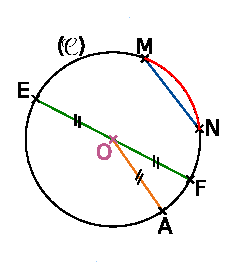
\includegraphics[width=\linewidth]{cCD01}} & Un \textbf{rayon} d'un cercle est un segment ayant pour extrémités le centre et un point de ce cercle. & Le segment $[OA]$ est un \textbf{rayon} du cercle $(\mathcal{C})$.  \\ \cline{2-3}
     & Un \MotDefinition{diamètre}{} d'un cercle est un segment ayant pour extrémités deux points de ce cercle et contenant son centre. & Le segment $[EF]$ est un \textbf{diamètre} du cercle $(\mathcal{C})$. \\ \cline{2-3}
     & Une \MotDefinition{corde}{} d'un cercle est un segment ayant pour extrémités deux points de ce cercle. & Le segment $[MN]$ est une \textbf{corde} du cercle $(\mathcal{C})$. \\ \cline{2-3}
     & Un \MotDefinition{arc de cercle}{} est une portion de cercle comprise entre deux points de ce cercle. & La portion de cercle $\overset{\frown}{MN}$ comprise entre $M$ et $N$ est un \textbf{arc du cercle} $(\mathcal{C})$. \\ \hline
     & Un \MotDefinition{disque}{} est une région du plan limitée par un cercle. &  \\ \cline{2-3}
     & Un \MotDefinition{secteur circulaire}{} est une partie du disque comprise entre deux rayons. &  \\ \hline
\end{tabular}

 
\begin{remarque}
Par commodité de langage, on appelle \og rayon \fg la longueur du rayon d'un cercle, et on appelle \og diamètre \fg la longueur de son diamètre.
\end{remarque}

\begin{remarque}
Le diamètre d'un cercle est égal au double de son rayon.
\end{remarque}




\section{Périmètre du cercle}



\begin{definition}
Le \MotDefinition{périmètre (ou circonférence)}{} d'un cercle est \textbf{la longueur de son contour}.
\end{definition} 


\begin{propriete}
Si $R$ est le rayon d’un cercle et $D$ son diamètre, la circonférence du cercle est donnée par la formule :
\[ C = 2\cdot \pi \cdot R = \pi \cdot D \qquad \qquad \text{où } \pi= 3,1415926... \]
\end{propriete}



\begin{remarque}
Comme $\pi$ est un nombre infini, on utilise souvent, pour les calculs des valeurs approchées de $\pi$. L' approximation la plus fréquente est $\boldsymbol{\pi \approx 3,14}$.
\end{remarque}


\begin{exemple*1}
Le diamètre d'un cercle mesure 3 cm. Combien mesure sa circonférence ?

On prendra $\pi \approx 3,14$.
\correction
$C = \pi  \times D = 3,14 \times 3 = 9,42$. La circonférence du cercle est 9,42\,cm.
\end{exemple*1}


\begin{exemple*1}
Le rayon d'un cercle mesure 2\,cm. Combien mesure sa circonférence ?

On prendra $\pi \approx 3,14$.
\correction
 $C = 2 \times \pi \times R = 2 \times 3,14 \times 2 = 12,56$. La circonférence mesure 12,56\,cm.
\end{exemple*1}




\begin{exemple*1}
La circonférence d'un cercle est de 15,7\,cm. Quel en est le diamètre ?
\correction
$C = \pi \times D$ donc $15,7 = 3,14 \times D$ d'où on tire $D = 15,7 \div 3,14 = 5$.

Le diamètre mesure 5\,cm.
\end{exemple*1}
 	 

		
		
		
\section{Aire du disque}



\begin{propriete}
L'\MotDefinition{aire d'un disque}{} de rayon $R$ est donnée par la formule :
\[ \mathcal{A} = \pi \times R \times R = \pi R^2 \]
\end{propriete} 
 

\begin{exemple*1}
Calculer l'aire $\mathcal{A}$ d'un disque de rayon $4,8$\,dm. Donner la valeur arrondie au cm\up{2}.
\correction
$A = \pi R^2 = \pi \times 4,82 = 3,14 \times 23,04 \approx 72,345$.

L'aire du disque est donc égale à 7 235\,cm\up{2}. 
\end{exemple*1}




\section{Calculer une aire par découpage}


\begin{exemple*1}
Calculer l’aire de la figure suivante :

\begin{center}
    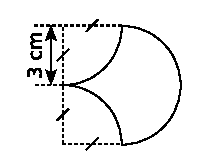
\includegraphics[width=.2\linewidth]{cCD02}
\end{center}

\correction
Pour calculer l'aire de cette figure, on découpe la figure en trois morceaux puis on les déplace pour reconstituer une figure connue.

\begin{center}
    \hfill 
\includegraphics[width=.15\linewidth]{cCD03} \hfill 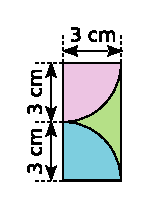
\includegraphics[width=.15\linewidth]{cCD04} \hspace*{\fill}
\end{center}
						
Calculer l'aire de cette figure revient donc à calculer l'aire d'un rectangle de largeur 3\,cm et de longueur 6\,cm : $\mathcal{A} = 3 \text{cm} \times 6 \text{cm} = 18$\,cm\up{2}.

L'aire de cette figure est 18\,cm\up{2}.
\end{exemple*1}



\begin{exemple*1}
Calculer l'aire de la figure suivante.
\begin{center}
    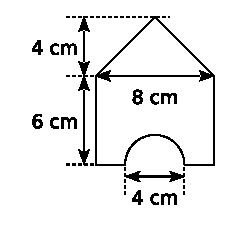
\includegraphics[width=.25\linewidth]{cCD05}
\end{center}
\correction
Pour calculer l'aire de cette figure, on repère des figures simples qui la constituent...
\begin{center}
    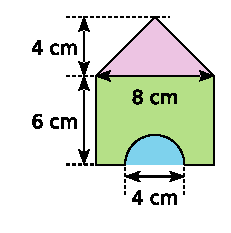
\includegraphics[width=.25\linewidth]{cCD06}
\end{center}
... puis on calcule l'aire de chacune des figures simples trouvées.

\vspace{1em}

\begin{tabular}{p{.32\linewidth}|p{.32\linewidth}|p{.32\linewidth}}
Un \textbf{triangle} dont un côté mesure 8\,cm et la hauteur relative à ce côté mesure 4\,cm. & Un \textbf{rectangle} de largeur 6\,cm et de longueur 8\,cm. & Un \textbf{demi-disque} de rayon 2\,cm. \\
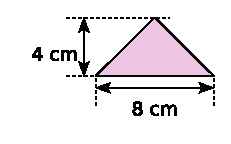
\includegraphics[width=.7\linewidth]{cCD07} & 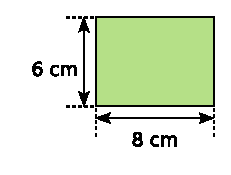
\includegraphics[width=.7\linewidth]{cCD08} & \hspace*{.3\linewidth}
\includegraphics[width=.3\linewidth]{cCD09}\\
  $\mathcal{A}_T = \dfrac{8 \times 4}{2}= 16$\,cm\up{2} & $\mathcal{A}_R = 6 \times 8 = 48$\,cm\up{2} & $\mathcal{A}_D =\dfrac{\pi \times 2^2}{2}= 2\pi$\,cm\up{2} \\
\end{tabular}

\vspace{1em}

L'aire de la figure est obtenue en additionnant l'aire du triangle et du rectangle puis en retranchant au résultat l'aire du demi-disque :
\[ \mathcal{A}= \mathcal{A}_T + \mathcal{A}_R - \mathcal{A}_D = 16 \text{ cm\up{2}} + 48 \text{ cm\up{2}} - 2\pi \text{ cm\up{2}} = 64 - 2\pi \text{ cm\up{2}}. \]

L'aire exacte de cette figure est $64 - 2\pi$\,cm\up{2}.

En prenant 3,14 comme valeur approchée du nombre $\pi$, on obtient $\mathcal{A} \approx 57,72$\,cm\up{2}.
\end{exemple*1}



\begin{exemple*1}
Calculer l'aire de chacune des figures suivantes :
\begin{center}
    \hfill 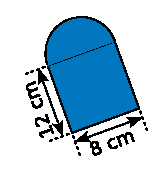
\includegraphics[width=.2\linewidth]{cCD10} \hfill 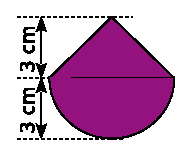
\includegraphics[width=.2\linewidth]{cCD11} \hspace*{\fill}
\end{center}
%\correction

\end{exemple*1}

							


\exercicesbase
\begin{colonne*exercice}
\serie{Calculer l'aire d'un parallélogramme}



\begin{exercice}[Avec un quadrillage]
Sachant que l'unité d'aire est le carreau, détermine l'aire de chaque figure suivante en utilisant des aires de parallélogrammes.
\begin{center}
    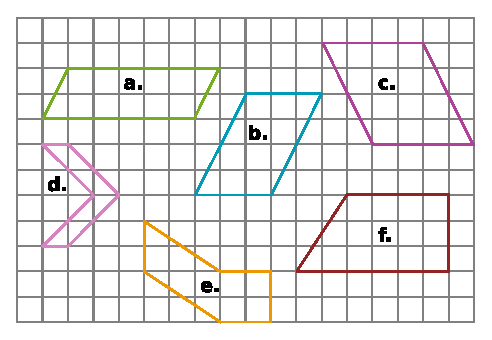
\includegraphics[width=\linewidth]{eeCD01}
\end{center}
\end{exercice}



\begin{exercice}[]
Calcule l'aire de chaque parallélogramme dont les dimensions sont données ci-dessous.
\begin{colenumerate}{1} 
\item Un côté mesure 6\,cm et la hauteur relative à ce côté mesure 4\,cm.
\item Un côté mesure 4,7\,dm et la hauteur relative à ce côté mesure 7,2\,cm.
\item Un côté mesure 2\,m et la hauteur relative à ce côté mesure 6,4\,cm.
\end{colenumerate} 
\end{exercice}

\begin{exercice}[]
Calcule la longueur demandée.
\begin{colenumerate}{1} 
\item L'aire du parallélogramme est 36\,cm\up{2} et l'un de ses côtés mesure 6\,cm. Combien mesure la hauteur relative à ce côté ?
\item L'aire du parallélogramme est 15,12\,cm\up{2} et l'une de ses hauteurs mesure 3,6\,cm. Combien mesure le côté associé à cette hauteur ?
\end{colenumerate} 
 
\end{exercice}

\begin{exercice}[Ne pas confondre !]
Calcule l'aire et le périmètre de ce parallélogramme tracé à main levée.
\begin{center}
    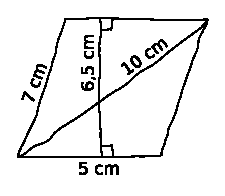
\includegraphics[width=.5\linewidth]{eeCD02}
\end{center}

\end{exercice}

\begin{exercice}[L'un dans l'autre]
Sur la figure suivante, les points $V$, $E$, $L$ et $U$ sont les milieux des côtés d'un rectangle $RATO$.

\begin{colenumerate}{1} 
\item Calcule l'aire de $RATO$, sachant que $RA =$8\,cm et $AT =$6\,cm.
\item Calcule l'aire de $VELU$ de deux façons.
\end{colenumerate} 

\begin{center}
    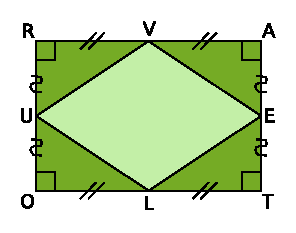
\includegraphics[width=.65\linewidth]{eeCD03}
\end{center}
 
\end{exercice}



\serie{Calculer l'aire d'un triangle}






\begin{exercice}[Avec un quadrillage (bis)]
Sachant que l'unité d'aire est le carreau, détermine l'aire des figures suivantes en utilisant des aires de triangles.

\begin{center}
    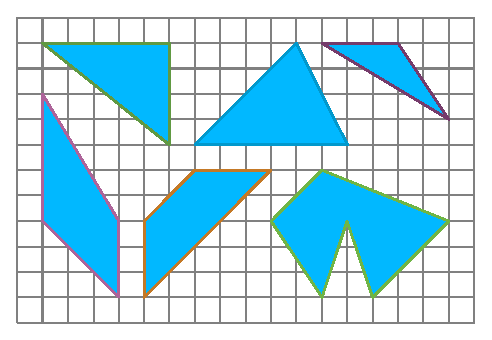
\includegraphics[width=\linewidth]{eeCD04}
\end{center}

\end{exercice}

\begin{exercice}[Calculer (mentalement !) pour construire]

\begin{colenumerate}{1} 
\item Trace un triangle $OIL$ rectangle en $O$ d'aire 15\,cm\up{2}.
\item Trace un triangle isocèle $EAU$ d'aire 12\,cm\up{2}.
\end{colenumerate} 
\end{exercice}



\begin{exercice}[]
En utilisant les données de l'énoncé, calcule l'aire du triangle $DEF$ puis déduis-en les longueurs $DK$ et $DF$.

\ImageDroite{$DE = 8$\,cm

	$EF = 5$\,cm
	
	$IF = 2,1$\,cm
	
	$EJ = 4,2$\,cm
	}{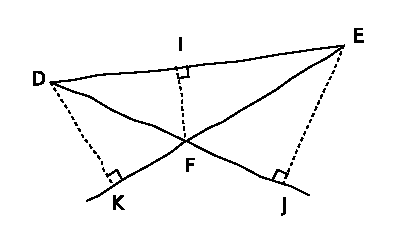
\includegraphics[width=.6\linewidth]{eeCD05}}
\end{exercice}



\serie{Cercles}



\begin{exercice}[Comparaison]

\begin{colenumerate}{1} 
\item Compare le périmètre de ces quatre figures. 

\begin{center}
    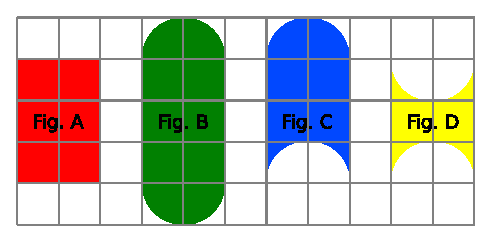
\includegraphics[width=\linewidth]{eeCD06b}
\end{center}
\item Compare l'aire de ces quatre figures. Justifie.
\end{colenumerate} 
\end{exercice}


\begin{exercice}[]
Calcule le périmètre des cercles suivants. Tu donneras la valeur exacte puis une valeur approchée au centième près.  

\begin{center}
    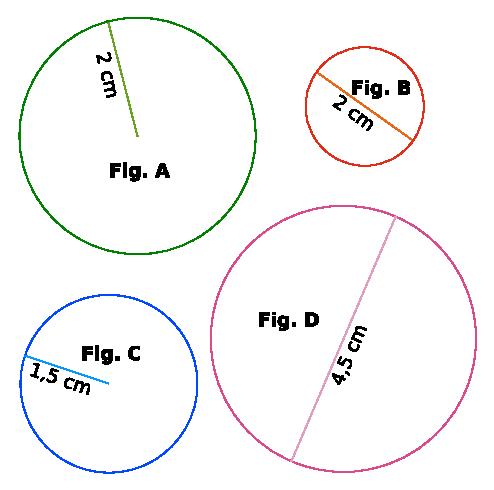
\includegraphics[width=\linewidth]{eeCD07}
\end{center}
\end{exercice}


\begin{exercice}[Trio de figures]

\begin{colenumerate}{1} 
\item Vincent affirme que les trois figures ci-dessous ont le même périmètre. A-t-il raison ?
 
\begin{center}
    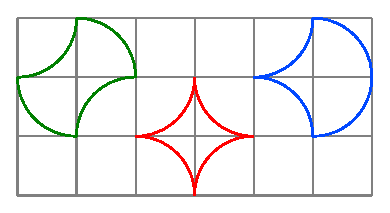
\includegraphics[width=.85\linewidth]{eeCD08}
\end{center}

\item Chaque carré a pour côté 1\,cm. Calcule le périmètre de ces trois figures.
\end{colenumerate} 
 
\end{exercice}

\begin{exercice}[]
Calcule le périmètre des cercles suivants. Tu donneras la valeur exacte puis une valeur approchée au dixième.

\begin{colenumerate}{2} 
\item Rayon : 3\,cm 
\item Rayon : 4,5\,cm
\item Rayon : 5\,dm
\item Diamètre : 7\,cm
\item Diamètre : 8\,cm
\item Diamètre : 25\,mm
\end{colenumerate} 
\end{exercice}

\begin{exercice}[]
On considère que l'équateur est un cercle de rayon 6 400\,km. Calcule le périmètre de l'équateur. Donne une valeur approchée au millier de kilomètres près.
\end{exercice}

\begin{exercice}[]
Calcule le périmètre de l'intérieur du stade Gerland de Lyon (il est constitué d'un rectangle et de deux demi-cercles). Tu donneras la valeur exacte et une valeur approchée au centimètre.

\begin{center}
    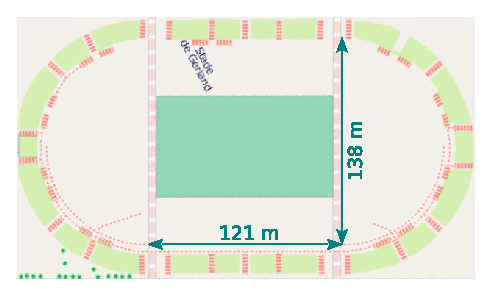
\includegraphics[width=\linewidth]{eeCD09}
\end{center}
\end{exercice}


\begin{exercice}[]
\ImageDroite{Une grande roue d'une fête foraine a un diamètre de 38\,m. Donne une valeur approchée au dixième de...}{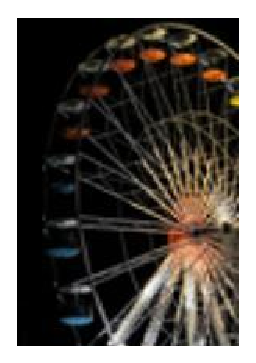
\includegraphics[width=.3\linewidth]{roue}}

\hfill {\scriptsize \textit{Source : Wikimedia Commons}}


\begin{colenumerate}{1} 
\item ... la distance parcourue en un tour de grande roue ;
\item ... la distance parcourue en cinq tours de grande roue.
\end{colenumerate} 
\end{exercice}



\serie{Conversions}




\begin{exercice}[]
Recopie et complète.

\begin{colenumerate}{2} 
\item 4\,dam\up{2} = ... m\up{2}
\item 15\,hm\up{2} = ... m\up{2}
\item 5,1\,cm\up{2} = ... mm\up{2}
\item 1 350\,mm\up{2} = ... cm\up{2}
\item 5,2\,km\up{2} = ... m\up{2}
\item 0,7\,m\up{2} = ... dam\up{2}
\item 320\,a = ... m\up{2}
\item 2,5\,ha = ...m\up{2}
\item 15 300\,mm\up{2} = ... cm\up{2} = ... dm\up{2} = ... m\up{2}
\end{colenumerate} 
\end{exercice}

\begin{exercice}[]
Convertis les aires suivantes en m\up{2}.

\begin{colenumerate}{3} 
\item 2\,km\up{2}
\item 37 000\,dm\up{2}
\item 45 300\,mm\up{2}
\item 153,7\,dam\up{2}
\item 28,9\,cm\up{2}
\item 3,008\,hm\up{2}
\item 52\,a
\item 0,05\,ha
\item 200\,ha
\end{colenumerate} 
\end{exercice}


\begin{exercice}[]
Convertis les aires suivantes en cm\up{2}.

\begin{colenumerate}{3} 
\item 15\,mm\up{2}
\item 28\,dm\up{2}
\item 17 300\,mm\up{2}
\item 73,1\,m\up{2}
\item 0,004\,m\up{2}
\item 27,008\,dam\up{2}
\item 0,08\,mm\up{2}
\item 13\,a
\item 0,0105\,a
\end{colenumerate} 
 
\end{exercice}

\begin{exercice}[]
On  donne les superficies suivantes :
\begin{itemize}
    \item Belle-Île-en-mer : 90\,km\up{2}
    \item Île d’Yeu : 2 300\,ha
    \item Île d’Oléron : 175 000 000\,m\up{2}
    \item Île de Jersey : 1 160 000\,dam\up{2}
\end{itemize}

Range ces îles dans l’ordre décroissant de leur superficie.   
\end{exercice}

\begin{exercice}[]
Un jardinier est chargé de la décoration d'un rond-point de 10 mètres de rayon.

\begin{colenumerate}{1} 
\item Il souhaite planter du gazon sur l'intégralité du rond-point. Quelle quantité doit-il prévoir ?
\item Il souhaite planter des fleurs sur le bord extérieur du rond-point, tous les 20\,cm. Combien doit-il prévoir de pots de fleurs ?
\end{colenumerate} 
\end{exercice}



\begin{exercice}[]
Le lac Pavin est un lac français situé dans le Massif Central. Il occupe le cratère presque circulaire d'un ancien volcan. Son diamètre est de 750\,m. 

\begin{colenumerate}{1} 
\item Calcule le périmètre de ce lac. Donne une valeur approchée au mètre près.
\item Calcule l'aire du lac. Donne une valeur approchée à l'hectare près.
\end{colenumerate} 

\end{exercice}



\serie{Disques}



\begin{exercice}[]
Calcule l'aire de chaque disque. Tu donneras la valeur exacte puis une valeur approchée au dixième.

\begin{colenumerate}{2} 
\item Rayon : 4\,cm
\item Rayon : 6\,dm
\item Diamètre : 1,5\,mm 
\item Diamètre : 10,3\,m
\end{colenumerate} 
\end{exercice}

\begin{exercice}[]
Calcule l'aire de chaque disque. Tu donneras la valeur exacte puis une valeur approchée au dixième.

\begin{center}
    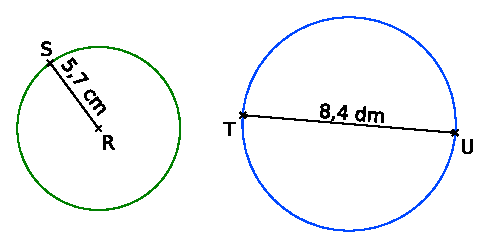
\includegraphics[width=\linewidth]{eeCD11}
\end{center}
\end{exercice}

\begin{exercice}[]
Calcule l'aire de cette figure sachant que sa largeur dans la réalité est de 6,4\,cm.

\begin{center}
    
\includegraphics[width=.6\linewidth]{eeCD12}
\end{center}
\end{exercice}


\begin{exercice}[]
Effectue les calculs suivants.

\begin{colenumerate}{1} 
\item L'aire exacte d'un disque de rayon 3\,cm.
\item Une valeur approchée au dixième près de l'aire d'un disque de rayon 35\,mm.
\item L'aire exacte d'un disque de diamètre 8\,cm.
\end{colenumerate} 
\end{exercice}


\begin{exercice}[]
Donne la valeur exacte puis la valeur approchée au centième près de l'aire des disques suivants, où $r$ désigne le rayon du disque et $d$ le diamètre du disque.

\begin{colenumerate}{3} 
\item $r$ = 2\,cm
\item $d$ = 3\,cm
\item $r$ = 4,5\,cm
\item $r$ = 5,6\,cm
\item $d$ = 4,8\,dm
\item $d$ = 0,24\,m
\end{colenumerate} 
 
\end{exercice}

\begin{exercice}[]
Calcule l'aire de chaque figure suivante.
\begin{center}
    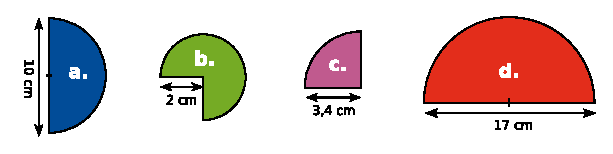
\includegraphics[width=\linewidth]{eeCD13}
\end{center}
\end{exercice}



\begin{exercice}[Portions de disques]

\begin{colenumerate}{1} 
\item Calcule l'aire d'un demi-disque de rayon 5,2\,cm. Donne la valeur exacte puis une valeur approchée au mm\up{2} près.
\item Calcule l'aire d'un quart de disque de rayon 16,4\,cm. Donne la valeur exacte puis une valeur approchée au mm\up{2} près.
\end{colenumerate} 
 
\end{exercice}

\begin{exercice}[]
Recopie et complète le tableau. (On prendra 3,14 comme valeur approchée de $\pi$.)

\renewcommand*\tabularxcolumn[1]{>{\centering\arraybackslash}m{#1}}
\begin{ltableau}{\linewidth}{4}
\hline
Rayon & Diamètre & Périmètre & Aire \\ \hline
5\,cm &   &   &   \\ \hline
 & 2,4\,dm  &   &   \\ \hline
 &   &  6,28\,m &   \\ \hline
 &   &   & 50,24\,cm\up{2}  \\ \hline
\end{ltableau}
\end{exercice}




\begin{exercice}[]
À Mathcity, l'émetteur de \og Radio-Centre \fg a une portée de 10\,km.


\begin{colenumerate}{1} 
\item Calcule la superficie de la zone de réception au km\up{2} près.
\item À partir du mois de septembre prochain, le conseil municipal instaure une taxe de 10 € par km\up{2}. Combien paiera \og radio-centre \fg ?
\item La direction prévoit de changer l'émetteur pour multiplier la portée par 3. La nouvelle taxe sera-t-elle aussi multipliée par 3 ? 
\end{colenumerate} 
\end{exercice}

\begin{exercice}[]
Calcule l'aire et le périmètre de ce stade.
\begin{center}
    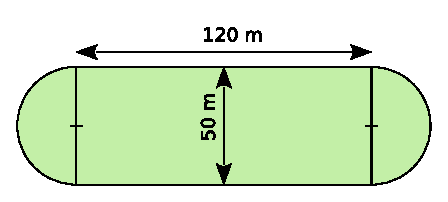
\includegraphics[width=.8\linewidth]{eeCD17}
\end{center}

\end{exercice}

\begin{exercice}[Quadrillage]

\begin{center}
    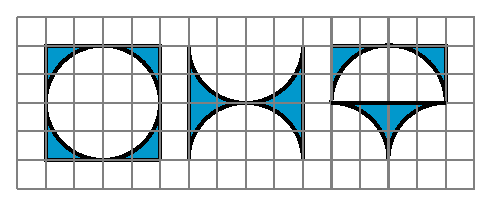
\includegraphics[width=\linewidth]{eeCD18}
\end{center}

Reproduis les figures ci-dessus dans des carrés de 4\,cm de côté puis calcule l'aire de chaque surface coloriée.
\end{exercice}

\end{colonne*exercice}


\exercicesappr
\begin{colonne*exercice}

\begin{exercice}[]
Calcule le périmètre et l'aire de la plaque métallique représentée ci‑dessous.

\begin{center}
    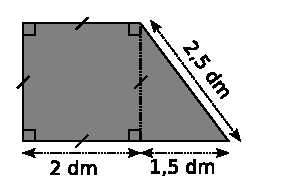
\includegraphics[width=.5\linewidth]{eaCD01}
\end{center}
\end{exercice}



\begin{exercice}[]
La figure suivante représente un morceau de tissu. Calcule son aire.
\begin{center}
    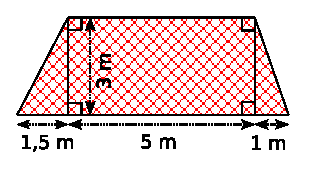
\includegraphics[width=.66\linewidth]{eaCD02}
\end{center}
\end{exercice}

\begin{exercice}[]
On souhaite entourer, avec du grillage, un jardin carré de 24\,m de côté, en laissant une ouverture de 4\,m de large. Le grillage choisi coûte 15\,€ le mètre. Quel sera le prix à payer ?
\end{exercice}

\begin{exercice}[]
M. Albert vend un terrain représenté ci‑dessous, au prix de 18\,€ le m\up{2}.

\begin{center}
    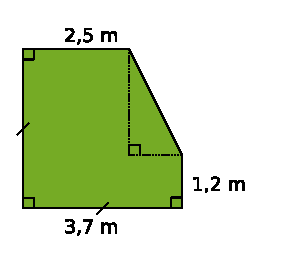
\includegraphics[width=.4\linewidth]{eaCD03}
\end{center}

Quel est le prix de vente de ce terrain ?
\end{exercice}

\begin{exercice}[]
Donne une valeur approchée au dixième du périmètre et de l'aire de la figure.

\begin{center}
    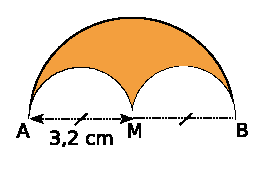
\includegraphics[width=.5\linewidth]{eaCD04}
\end{center}
\end{exercice}

\begin{exercice}[]
Donne la valeur approchée par excès à l'unité du périmètre et de l'aire de la partie jaune.
\begin{center}
    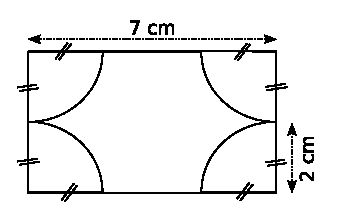
\includegraphics[width=.7\linewidth]{eaCD05}
\end{center}
\end{exercice}

\begin{exercice}[]
Dans une pièce de bois rectangulaire de dimensions 10,2\,cm sur 6,6\,cm, un menuisier découpe un losange. Il perce ensuite, au centre de ce losange, un trou circulaire de 1\,cm de diamètre.

\begin{center}
    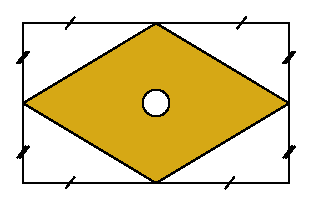
\includegraphics[width=.7\linewidth]{eaCD06}
\end{center}

Donne un arrondi à l'unité de l'aire de la pièce de bois obtenue.
\end{exercice}

\begin{exercice}[]
Un massif circulaire a un diamètre de 10\,m. On souhaite y planter 50 rosiers régulièrement espacés, à 30\,cm du bord. Quelle distance y aura‑t‑il entre chaque plant ? (Donne le résultat arrondi au centimètre.)
\end{exercice}

\begin{exercice}[]
Un artisan rénove une pièce de 3,50\,m de largeur, 4\,m de longueur et 2,50\,m de hauteur. 

\begin{colenumerate}{1} 
\item Sur le plafond, il met deux couches de peinture. Un pot de peinture permet de couvrir 6\,m\up{2}. De combien de pots a-t-il besoin ?
\item Il tapisse tous les murs avec du papier peint. Chaque rouleau est large de 50\,cm et long de 10\,m, sans raccord. Combien de rouleaux doit-il prévoir ? On ne tiendra pas compte des ouvertures (portes et fenêtres).
\end{colenumerate} 
\end{exercice}

\begin{exercice}[]
Construis un parallélogramme qui a un côté de 6\,cm de longueur, un périmètre de 20\,cm et une aire de 18\,cm\up{2}. Justifie ta construction en indiquant tes calculs.
\end{exercice}

\begin{exercice}[Attention travaux !]
Un peintre en bâtiment fait l’expérience suivante : il imbibe entièrement son rouleau de peinture, il le pose sur le mur, le fait rouler en lui faisant faire seulement un tour complet, puis le retire du mur.

\begin{colenumerate}{1} 
\item Quelle va être la forme de la tache de peinture ainsi réalisée ?
\item Le rouleau est large de 25\,cm et d’un diamètre de 8\,cm. Quelle surface du mur sera alors recouverte de peinture ?
\item Combien de fois, au minimum, devra-t-il réaliser ce geste pour peindre un mur long de 6\,m et haut de 2,5\,m ?
\end{colenumerate} 
\end{exercice}


\begin{exercice}[La galette]
Un pâtissier doit confectionner une tarte recouverte de glaçage. Il sait qu'avec 100\,g de sucre glace, il fabrique du glaçage pour une surface de 5\,dm\up{2}. Sachant qu'il dispose de moules à tarte circulaires de diamètres 22\,cm, 26\,cm ou 28\,cm, quel moule devra-t-il utiliser pour 100\,g de sucre ?
\end{exercice}

\begin{exercice}[Le nautile]
\ImageDroite{Le nautile est un mollusque dont la coquille est spiralée et peut être schématisée de la manière suivante.}{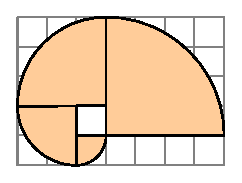
\includegraphics[width=.4\linewidth]{eaCD07}}

\begin{colenumerate}{1} 
\item Reproduis ce schéma dans un quadrillage à carreaux de 1\,cm de côté.
\item Calcule l'aire de la figure.
\item Calcule le périmètre de cette figure.
\end{colenumerate} 
\end{exercice}



\begin{exercice}[Une couronne pour un roi]
\ImageDroite{Calcule l'aire de la couronne circulaire ci-contre en arrondissant le résultat au mm\up{2} le plus proche.}{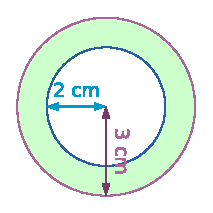
\includegraphics[width=.4\linewidth]{eaCD08}}
\end{exercice}


\begin{exercice}[] 
quadrilatère ABCD est un rectangle tel que $BC = 4$\,cm, $AB = 6$\,cm et $K$ est le milieu de $[AD]$. La surface colorée est formée de parallélogrammes accolés. Montre que l'aire de la surface colorée est la moitié de celle du rectangle.
\begin{center}
    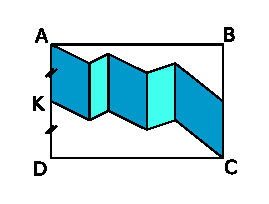
\includegraphics[width=.5\linewidth]{eaCD09}
\end{center}
\end{exercice}

\begin{exercice}[Pare-brise]
Sur un pare-brise rectangulaire de 1,50\,m par 0,80\,m est fixé (au milieu de la longueur) un essuie-glace de longueur 0,65\,m. Trouve une valeur approchée du pourcentage de la surface balayée par rapport à celle du pare-brise.
\end{exercice}


\begin{exercice}
\ImageDroite{On considère un cercle de rayon $r$\,cm ($r > 0$).}{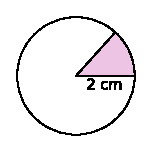
\includegraphics[width=.25\linewidth]{eaCD10}}

\begin{colenumerate}{1} 
\item\label{CDea1} On suppose ici que $r = 2$. Calcule l'aire de chaque secteur circulaire dont l'angle est donné dans le tableau suivant.

\vspace{1em}

% la commande de centrage des colonnes provoquent des erreurs ici
%\renewcommand*\tabularxcolumn[1]{>{\centering\arraybackslash}m{#1}}
{\footnotesize
\begin{ltableau}{\linewidth}{5}
\hline
Angle ($\circ$) & 360 & 90 & 45 & 180  \\ \hline
Aire (cm\up{2}) & & & &  \\ \hline
\end{ltableau}

\vspace{.5em}

\begin{ltableau}{\linewidth}{9}
\hline
Angle ($\circ$) & 120 & 3 & 1 & 12 \\ \hline
Aire (cm\up{2}) & & & & \\ \hline
\end{ltableau}
}% fin du footnotesize

\item Calcule le coefficient de proportionnalité du tableau précédent.
\item\label{CDea3} À l'aide du \ref{CDea1}, établis la formule donnant l'aire du secteur angulaire ci-dessous en faisant intervenir $x$, $r$ et le nombre $\pi$.

\begin{center}
    
\includegraphics[width=.25\linewidth]{eaCD11}
\end{center}

\item\label{CDea4} En utilisant la formule établie à la question \ref{CDea3}, calcule l'aire exacte des figures suivantes.

    \begin{center}
        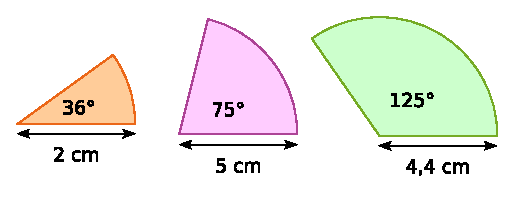
\includegraphics[width=\linewidth]{eaCD12}
    \end{center}
\item Déduis de la question \ref{CDea4} l'aire exacte :
    \subitem \textbullet d'un secteur angulaire de rayon 1\,cm et d'angle 111$^\circ$ ;
    \subitem \textbullet d'un secteur angulaire de rayon 8\,cm et d'angle 50$^\circ$.
\end{colenumerate} 
\end{exercice}


\begin{exercice}[Œuf de Pâques]
Voici un œuf de Pâques construit sur du papier pointé. L'unité est le centimètre. Le segment $[AO]$ mesure 4\,cm.

\begin{center}
    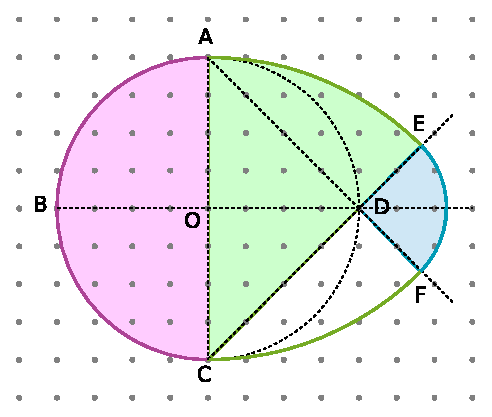
\includegraphics[width=\linewidth]{eaCD13}
\end{center}

\begin{center}\textbf{Construction}\end{center}

\begin{colenumerate}{1} 
\item Reproduis cette figure sur ton cahier. 
\item Propose un programme de construction pour cette figure.

\begin{center}\textbf{Les différentes parties de l'œuf}\end{center}

\item Cherche le rayon du demi-disque rose puis calcule son aire.
\item Cherche le rayon du huitième de disque vert puis calcule son aire.
\item Le segment $[AD]$ mesure 5,7\,cm. Cherche la longueur du segment $[DF]$ puis calcule l'aire du quart de disque bleu. 

\begin{center}\textbf{Aire de l'œuf}\end{center}


\item Un élève dit : \og Pour calculer l’aire de l'œuf, j’additionne l’aire de la partie rose, celle de la partie bleue et deux fois celle de la partie verte. \fg. A-t-il raison ? Sinon, explique.
\item Calcule l'aire du triangle rectangle $ADC$. 
\item Calcule alors une valeur approchée au dixième de l’aire de l'œuf.
 
\begin{center}\textbf{Un joli ruban}\end{center}

Marion veut entourer son œuf d'un joli ruban de laine en suivant le tour de l'œuf $AEFCBA$. 
\item Calcule une valeur approchée au dixième de la longueur de ruban nécessaire pour parer l'œuf de ce joli ruban.
\end{colenumerate} 
\end{exercice}

\begin{exercice}[]
Dans chaque cas, construis tous les quadrilatères qui satisfont aux énigmes suivantes.

\begin{colenumerate}{1} 
\item Je suis un quadrilatère dont les angles opposés sont égaux deux à deux. Mon aire vaut 28\,cm\up{2} et mon périmètre 24\,cm. Mes côtés ont des mesures entières.
\item Je suis un parallélogramme dont les diagonales sont de même longueur. La connaissance soit de la longueur d’une diagonale, soit d’un de mes côtés suffit pour que l’on puisse calculer mon aire qui est égale à 8\,cm\up{2}.
\item Je suis un quadrilatère non croisé qui a deux côtés consécutifs égaux et qui possède ses diagonales perpendiculaires. Mon aire vaut 24\,cm\up{2}. Mes diagonales ont des mesures entières et mon centre se trouve au quart de la plus grande diagonale.
\end{colenumerate}
\end{exercice}

\end{colonne*exercice}

\connaissances
\QCMautoevaluation{Pour chaque question, plusieurs réponses sont proposées. Déterminer celles qui sont correctes.}

\begin{QCM}
\begin{GroupeQCM}

\begin{exercice}
L'aire d'un disque de diamètre 6\,cm est de...
\begin{ChoixQCM}{4}
\item $6\pi$ cm\up{2}
\item $36$ cm\up{2}
\item $9\pi$ cm\up{2}
\item $36\pi$ cm\up{2}
\end{ChoixQCM}

\begin{corrige}
\reponseQCM{a}
\end{corrige}
\end{exercice}

\begin{EnonceCommunQCM}
Les questions \RefQCM{CDqcmA} à \RefQCM{CDqcmB} se réfèrent à la figure ci-dessous :
\end{EnonceCommunQCM}

\begin{center}
    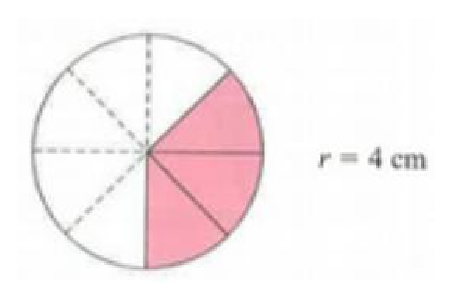
\includegraphics[width=.2\linewidth]{qcmCD01}
\end{center}

\begin{exercice}\label{CDqcmA}
L'aire du disque est :
\begin{ChoixQCM}{4}
\item $8\pi$ cm\up{2}
\item $4\pi^2$ cm\up{2}
\item $16\pi$ cm\up{2}
\item $16\pi$ cm
\end{ChoixQCM}

\begin{corrige}
\reponseQCM{a}
\end{corrige}
\end{exercice}



\begin{exercice}
L'aire du secteur angulaire rose (arrondie à 0,1 ) est :
\begin{ChoixQCM}{4}
\item $18,8$ cm\up{2}
\item $2,5$ cm\up{2}
\item $6,5$ cm\up{2}
\item $18,85$ cm\up{2}
\end{ChoixQCM}

\begin{corrige}
\reponseQCM{a}
\end{corrige}
\end{exercice}



\begin{exercice}\label{CDqcmB}
La circonférence du cercle est :

\begin{ChoixQCM}{4}
\item $8\pi$ cm
\item $4\pi^2$ cm
\item $16\pi$ cm
\item $8\pi$ cm\up{2}
\end{ChoixQCM}

\begin{corrige}
\reponseQCM{a}
\end{corrige}
\end{exercice}

\end{GroupeQCM}
\end{QCM}

\TravauxPratiques
%\input{CerclesDisques/CerclesDisques_enGrp.tex}

\recreation % avec R majuscule pour saut de page
\begin{enigme}[Tu vas au bal ?]

\ImageDroite{Sur le carton d'invitation rectangulaire ci‑contre, toutes les longueurs sont données en centimètres.

Quel est le code ?}%
{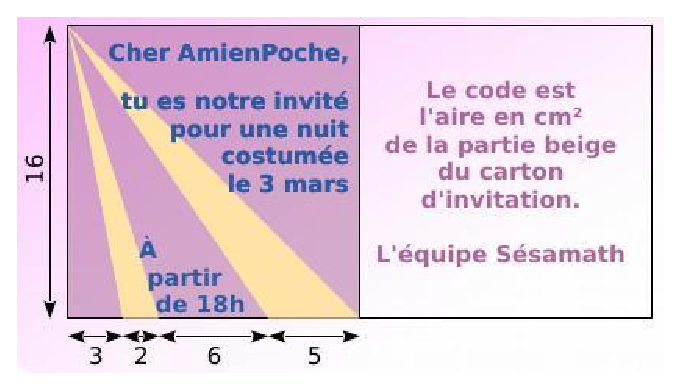
\includegraphics[width=.4\linewidth]{recCD01}}

\end{enigme}



